\documentclass[11pt]{article}
\usepackage{graphicx}
\begin{document}
\section{Ice Thermodynamics}
\label{Tphys}

\begin{figure}
\begin{picture}(0,0)%
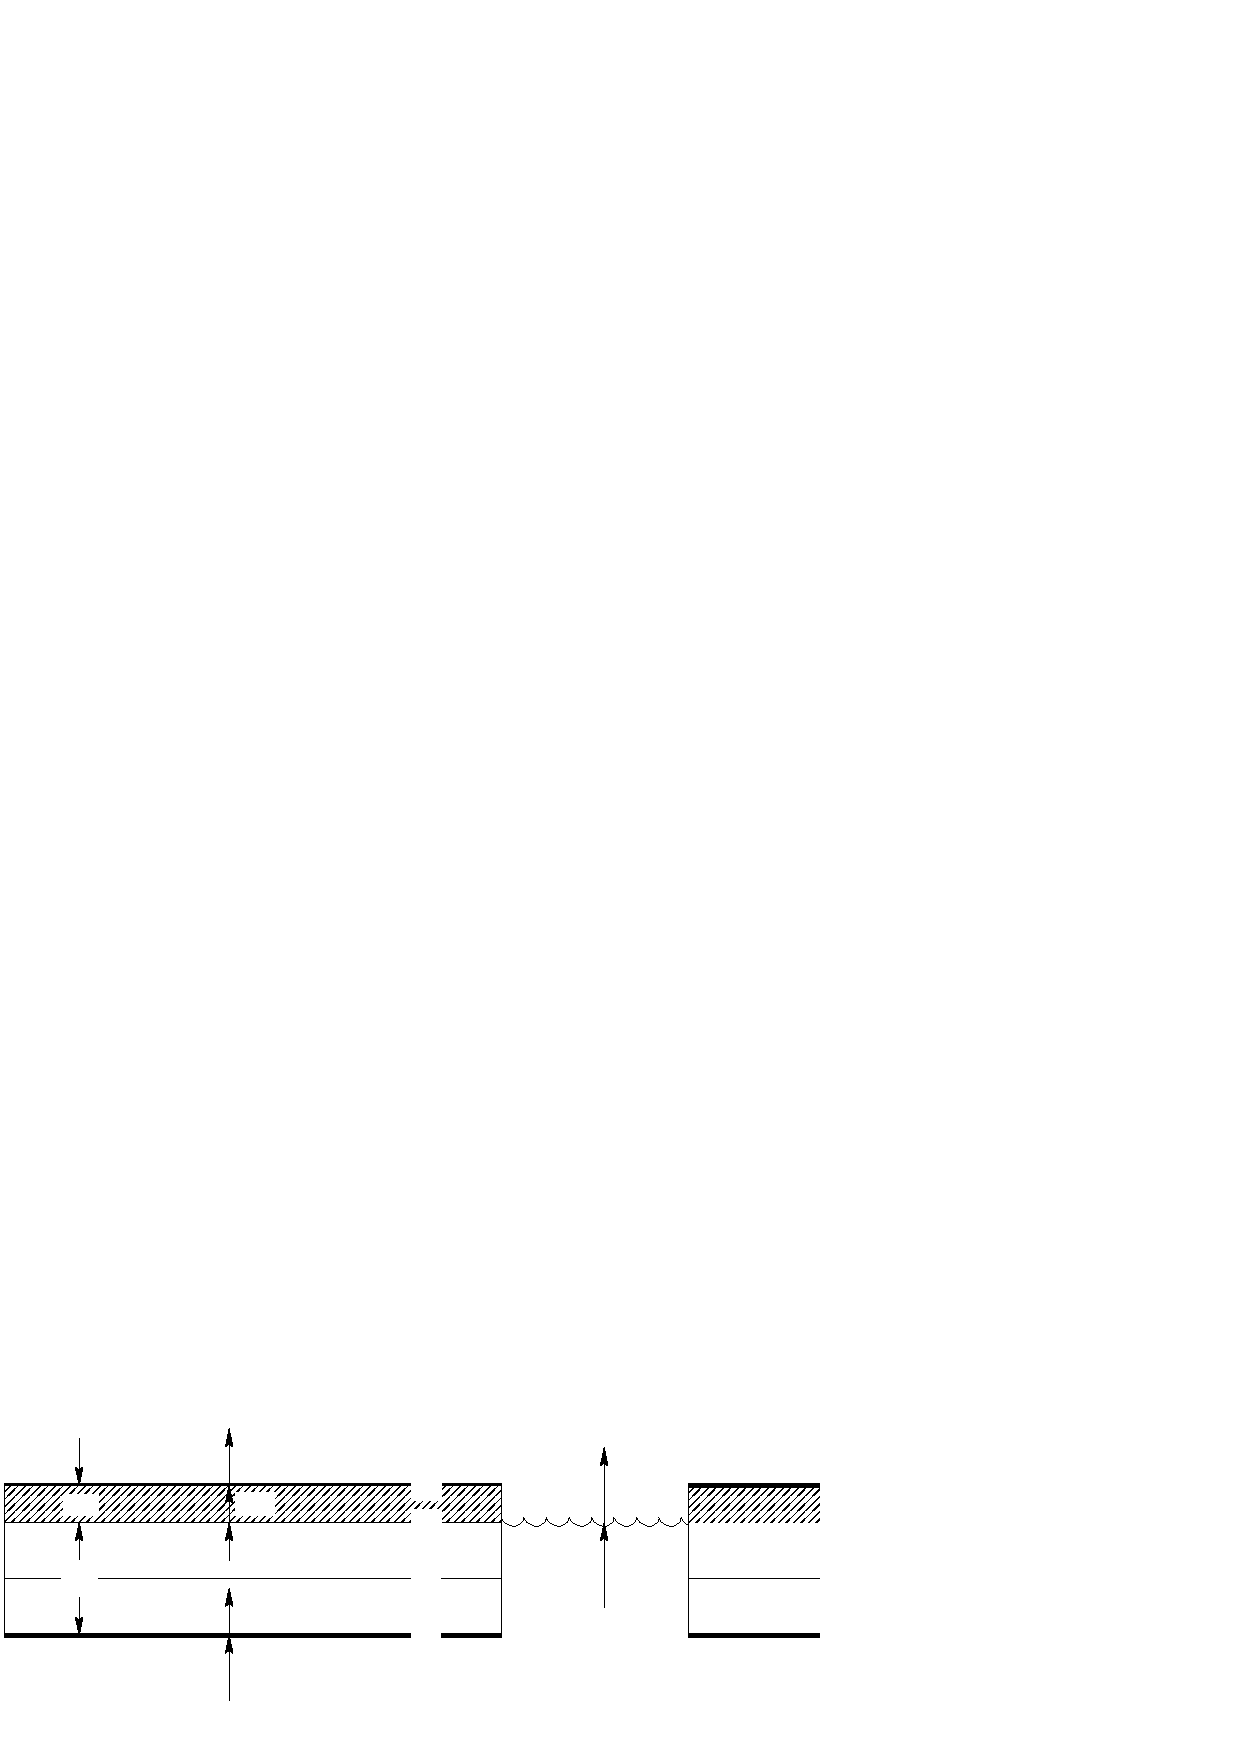
\includegraphics{pics/therm_mk2.pdf}%
\end{picture}%
\setlength{\unitlength}{3947sp}%
%
\begin{picture}(6591,2608)(1468,-5057)
\put(6376,-3511){\makebox(0,0)[lb]{{$F_T$}}}
\put(3376,-4561){\makebox(0,0)[lb]{{$F_T$}}}
\put(3376,-4036){\makebox(0,0)[lb]{{$Q_{IO}$}}}
\put(3376,-3436){\makebox(0,0)[lb]{{$Q_{I2}$}}}
\put(6376,-3061){\makebox(0,0)[lb]{{$Q_{AO}$}}}
\put(3376,-3136){\makebox(0,0)[lb]{{$Q_s$}}}
\put(3376,-2761){\makebox(0,0)[lb]{{$Q_{AI}$}}}
\put(2026,-3736){\makebox(0,0)[lb]{{$h_i$}}}
\put(2026,-3136){\makebox(0,0)[lb]{{$h_s$}}}
\put(4801,-4186){\makebox(0,0)[lb]{{$T_0$}}}
\put(4801,-2986){\makebox(0,0)[lb]{{$T_3$}}}
\put(4801,-3286){\makebox(0,0)[lb]{{$T_2$}}}
\put(4801,-3736){\makebox(0,0)[lb]{{$T_1$}}}
\end{picture}
\caption{Diagram of internal ice temperatures and fluxes (from MK89).}
\end{figure}

Inside the ice there are ``brine pockets'' in which there is salt water
at the {\it in situ} freezing temperature. It is assumed that the ice
has a uniform overall salinity of $S_i$ and that the freezing
temperature is a linear function of salinity. The brine fraction $r$ is
given by
$$
  r = {S_i m \over T_1}
$$
The enthalpy of the combined ice/brine system is given by
\begin{equation}
  E(T,r) = r(L_F + C_{po}T) + (1-r) C_{pi} T
\end{equation}
Substituting in for $r$ gives:
\begin{equation}
  {\partial E \over \partial T} = - {S_i m L_F \over T_1^2} + C_{pi}
\end{equation}

Inside the snow, we have
\begin{equation}
   Q_s = {k_s \over h_s} (T_2 - T_3)
\end{equation}
The heat conduction in the upper part of the ice layer is
\begin{equation}
   Q_{I2} = { 2 k_i \over h_i} (T_1 - T_2)
   \label{qi2}
\end{equation}
These can be set equal to each other to solve for $T_2$
\begin{equation}
   T_2 = {T_3 + C_k T_1 \over 1 + C_k}
\end{equation}
where
$$
  C_k \equiv {2 k_i h_s \over h_i k_s}.
$$
Substituting into (\ref{qi2}), we get:
\begin{equation}
  Q_{I2} = {2k_i \over h_i} {(T_1 - T_3) \over (1 + C_k)}
\end{equation}

At the bottom of the ice, we have
\begin{equation}
  Q_{I0} = {2 k_i \over h_i} (T_0 - T_1)
\end{equation}
The difference between $Q_{I0}$ and $Q_{I2}$ goes into the enthalpy of
the ice:
\begin{equation}
   \rho_i h_i \left[ {\partial E \over \partial t} + \vec{u} \cdot 
   \nabla E \right] = Q_{I0} - Q_{I2}
\end{equation}
We can use the chain rule to obtain an equation for timestepping $T_1$:
\begin{equation}
   \rho_i h_i {\partial E \over \partial T}
   \left[ {\partial T_1 \over \partial t} + \vec{u} \cdot 
   \nabla T_1 \right] = Q_{I0} - Q_{I2}
\end{equation}
where
\begin{eqnarray*}
  Q_{I0} - Q_{I2} & = & {2 k_i \over h_i} \left[ (T_0 - T_1) - 
  {(T_1 - T_3) \over 1 + C_k} \right] \\
	          & = & {2 k_i \over h_i} \left[ (T_0 +
  {T_3 - (2 + C_k) T_1 \over 1 + C_k} \right]
\end{eqnarray*}
\end{document}
